\section{1184071 - Annisa Khairani Febrianti}
\subsection{Teori}
\begin{enumerate}
	\item Definisi Kecerdasan Buatan (AI)
	\hfill\break
	Kecerdasan Buatan atau \textit{Artificial Intelligence} (AI) merupakan teknik meniru kecerdasan yang dimiliki oleh makhluk hidup maupun benda mati untuk menyelesaikan suatu masalah. Atau dapat di definisikan sebagai salah satu cabang Ilmu pengetahuan yang berkaitan dengan pemanfaatan mesin untuk menyelesaikan persoalan rumit dengan menggunakan cara yang lebih manusiawi. Adapun contoh sederhana penerapan kecerdasan buatan adalah SIRI, bagi pengguna iphone atau \textit{IOS} pasti sudah tidak asing dengan SIRI yang
    seringkali diartikan sebagai asisten pribadi pengguna IOS dalam melakukan hal-hal tertentu untuk penggunanya.

	\item Perkembangan dan Sejarah AI
	\hfill\break
	Pada tahun 1956 merupakan tahun pertama kali muncul istilah AI atau \textit{Artificial Intellegent} yang dikemukakan oleh \textbf{John McCarthy} di Konferensi Darthmouth.Penggunaan AI begitu popular dari tahun ke tahun. Pada tahun 1950-an merupakan tahap dimana riset awal proyek AI yang tujuan untuk eksplorasi topik penyelesaian persoalan dan metode simbolik.Selanjutnya Pada tahun 1959, Dari IBM yang bernama \textbf{Nathaniel Rochester} bersama beberapa mahasiswa lainnya mengeluarkan program kecerdasan buatan yaitu \textit{Geometry Theorm Prover}. Lalu pada tahun 1960-an Departemen Pertahanan yang berasal dari Amerika Serikat memiliki keinginan dalam melatih dan mengembangkan komputer supaya memiliki nalar yang menyerupai manusia secara dasar. Kemudian Pada tahun 1963, program yang mampu menyelesaikan masalah integral tertutup untuk mata kuliah Kalkulus dibuat dengan \textbf{James Slagle}. Pada tahun 1970-an, adanya suatu keberhasilan proyek DARPA \textit{(Defence Advanced Research Project Agency)} dengan mampu menyelesaikan studi kasus tentang pemetaan jalan. Selanjutnya Pada tahun 1986, program analogi yang digunakan dalam pemecahan masalah analogi geometris yang ada pada tes IQ dibuatan oleh \textbf{Tom Evan}. Dari tahun 1980an AI kemudian mulai berkembang dibidang idustri dan mulai berkiprah hingga saat ini dimana para ilmuan berlomba-lomba untuk menciptakan AI yang bermanfaat pada kehidupan sekarang atau dimasa depan nanti. Setelah itu pada awal abad ke 21 atau lebih tepatnya pada tahun 2003, DARPA berhasil untuk menciptakan asisten pribadi yang cerdas. Sejak saat itu lah teknologi AI terus berkembang sangat bagus dan sampai saat ini AI tersebutlebih menjurus pada program yang lebih detail dan kompleks dengan penerapan struktur algoritma dari pembelajaran secara mendalam atau \textit{deep learning} yaitu AI yang dikembangkan bisa mengerjakan persoalan dan memberi solusi yang lebih kompleks dengan kondisi yang lebih beragam.

	\item Kecerdasan buatan (AI) terbagi menjadi beberapa metode yaitu:
	\hfill\break
	Supervised learning,  Klasifikasi, Regresi,Unsupervised Learning, Dataset, Trainingset dan juga Testingset.
	\begin{itemize}
		\item Supervised Learning
		\hfill\break
	Supervised learning merupakan suatu pembelajaran dengan adanya pengawas atau bisa disebut dengan supervisor. Supervisor merupakan suatu label yang ada di setiap data nya. Kemudian label tersebut berisi tag dari data yang ditambah ke dalam model pembelajaran mesin atau lebih trend disebut dengan \textbf{machine learning model}. Bisa diilustrasikan seperti gambar apel di tag “apel” dari masing-masing gambar tersebut apel dan gambar pir di tag “pir”dari masing-masing gambar pir. Lalu Machine learning memiliki berapa kategori berupa clasification (“apel”, “pir”, dsb) dan regression ( tinggi badan, berat badan, dsb).
		\item Klasifikasi
		\hfill\break
		Klasifikasi merupakan sampel yang dimiliki oleh dua atau lebih kelas yang dikelompokkan yang disesuaikan berdasarkan ukuran kemiripan atau jarak yang melekat. 
		\item Regresi
		\hfill\break
    Regresi	merupakan sebuah prediksi apabila hasil atau output yang diinginkan terdiri dari satu atau lebih variable contionous.
		\item Unsupervised Learning 
		\hfill\break
Unsupervised learning merupakan suatu pembelajaran tanpa adanya sebuah pengawasan dan tidak menggunakan label untuk bisa memprediksi target variable. Unsupervised learning lebih mengelompokan tentang kesamaan ataupun kemiripan dari attribut yang sudah diinputkan. Apabila attribut dan sifat dari data variable yang diproses ternyata memiliki kemiripan, maka akan dijadikan
satu kelompok (clustering). Dan akan menimbulkan beberapa bagian kelompok (cluster). Jumlah cluster bisa tidak terbatas. Dari kelompok tersebut model melabelkan, dan jika data baru akan di prediksi, itu akan diproses untuk mencocokan kelompok yang memiliki kemiripan feature. unsupervised learning tidak punya outcome spesifik seperti supervise learning karena tidak adanya sebuah label dasar.
\hfill\break
\textbf{Dapat disimpulkan Jika Supervised learning tentang atribut atau label yang sudah ada dari kategori yang diinginkan berbeda dengan unservised learning dimana unsupervised menggunakan kesamaan dari attribut yang dimiliki. Jika attribut dan sifat dari data feature yang diekstrak memiliki
kemiripan, maka akan dikelompokan kedalam \textit{(clustering)}. Sehingga hal ini
akan menimbulkan kelompok \textit{(cluster)}. Jumlah cluster bisa unlimited atau tidak terbatas}.
		\item Data Set
		\hfill\break
Data Set merupakan kumpulan sampel yang sudah dikumpulkan dan bersifat
homogen. Salah satu contohnya yaitu Seorang anak ingin bermain Voli, tetapi keputusannya untuk bermain voli tersebut tergantung pada variable yang ditentukan contohnya jarak kaki dari garis, atau tinggi net sehingga variable ini disebut dengan fitur dalam sebuah permainan.
		\item Training Set
		\hfill\break
Data yang digunakan untuk bisa melakukan klasifikasi ataupun prediksi,Dengan adanya data training maka akan didapatkan sebuah model regresi.		
		\item Testing Set
		\hfill\break
Testing Set digunakan untuk menguji kebenaran dari sebuah model data.Adapun Testing data berisi \textit{unseen example} merupakan contoh yang tidak ada didalam training set.
	\end{itemize}
\end{enumerate}
\subsection{Praktek}
\begin{enumerate}
	\item Instalasi Library scikit dari Anaconda, mencoba kompilasi dan uji coba ambil contoh kode dan lihat variabel explorer
	\hfill\break
	\begin{figure}[h]
		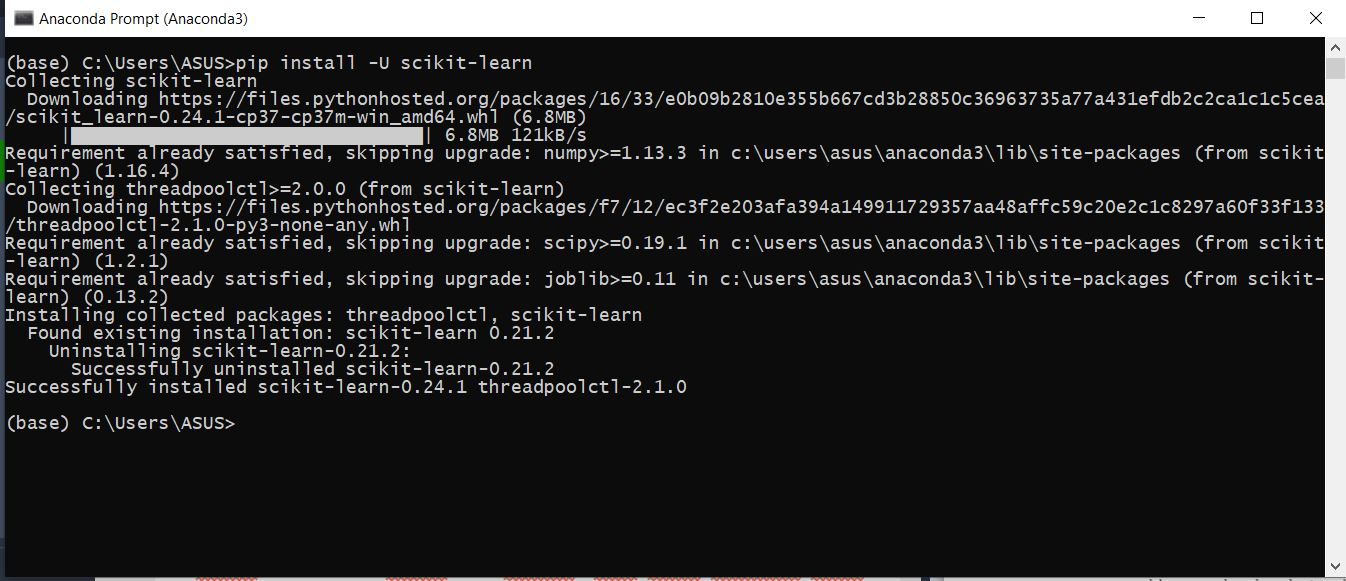
\includegraphics[width=12cm]{figures/1184071/chapter1/1.JPG}
		\centering
		\caption{Instalasi Library Scikit Learn}
	\end{figure}
	\begin{figure}[h]
		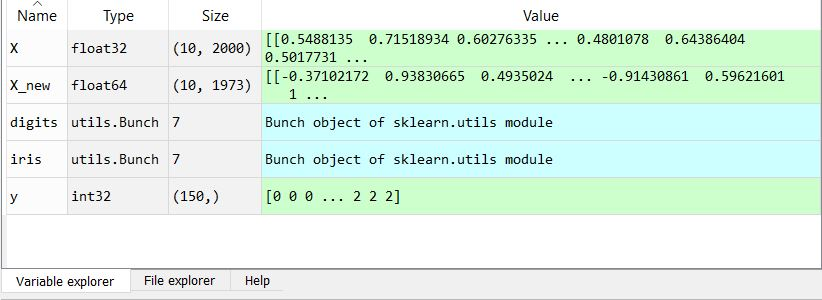
\includegraphics[width=15cm]{figures/1184071/chapter1/2.JPG}
		\centering
		\caption{Isi Variabel Explorer}
	\end{figure}
	\newpage\item Uji coba loading an example dataset
	\hfill\break
\lstinputlisting[firstline=7, lastline=16]{src/tugas1.py}
\item Uji coba Learning dan predicting
	\hfill\break
	\lstinputlisting[firstline=17, lastline=32]{src/tugas1.py}
\item Uji coba Model Persistence
	\hfill\break
	\lstinputlisting[firstline=35, lastline=63]{src/tugas1.py}	
	\item Uji coba Conventions
	\hfill\break
	\lstinputlisting[firstline=64, lastline=82]{src/tugas1.py}
	\end{enumerate}
	\subsection{Penanganan Error}
\begin{enumerate}
	\item ScreenShoot Error
	\begin{figure}[h]
		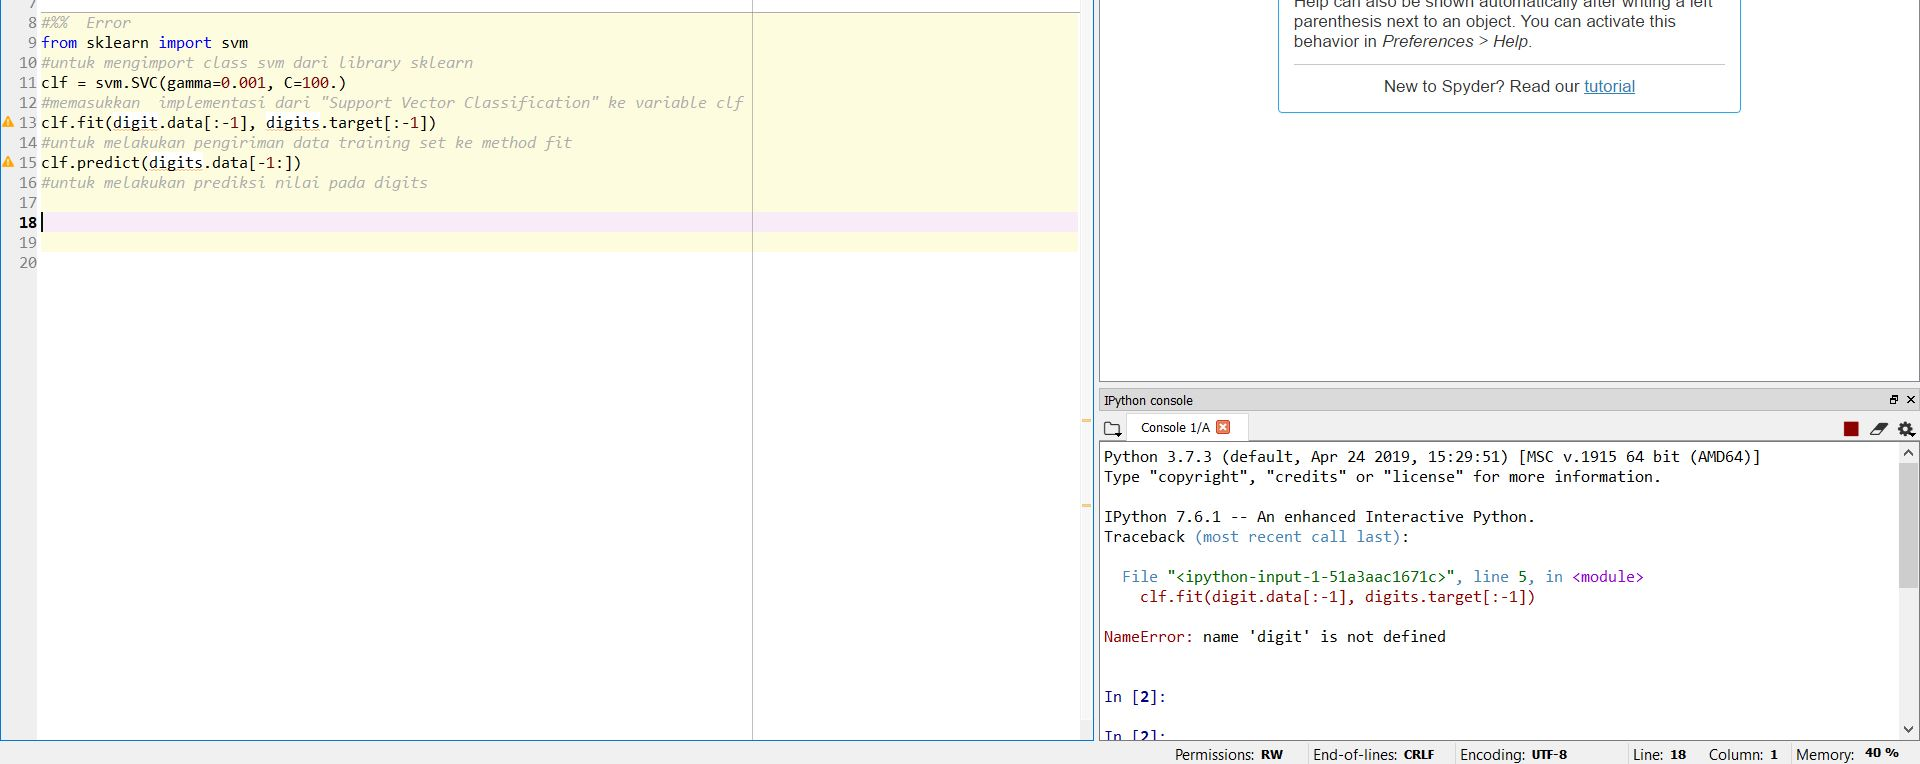
\includegraphics[width=15cm]{figures/1184071/chapter1/3.JPG}
		\centering
		\caption{Name Error}
	\end{figure}
	\newpage\item Tuliskan Kode Error dan Jenis Error
	\hfill\break
	\lstinputlisting[firstline=83, lastline=91]{src/tugas1.py}
\hfill\break
	\item Cara Penangan Error
\hfill\break Tambahkan variabel digits agar kode program dapat terbaca
	\end{enumerate}
	\subsection{Bukti Tidak Plagiarisme}
\begin{figure}[h]
	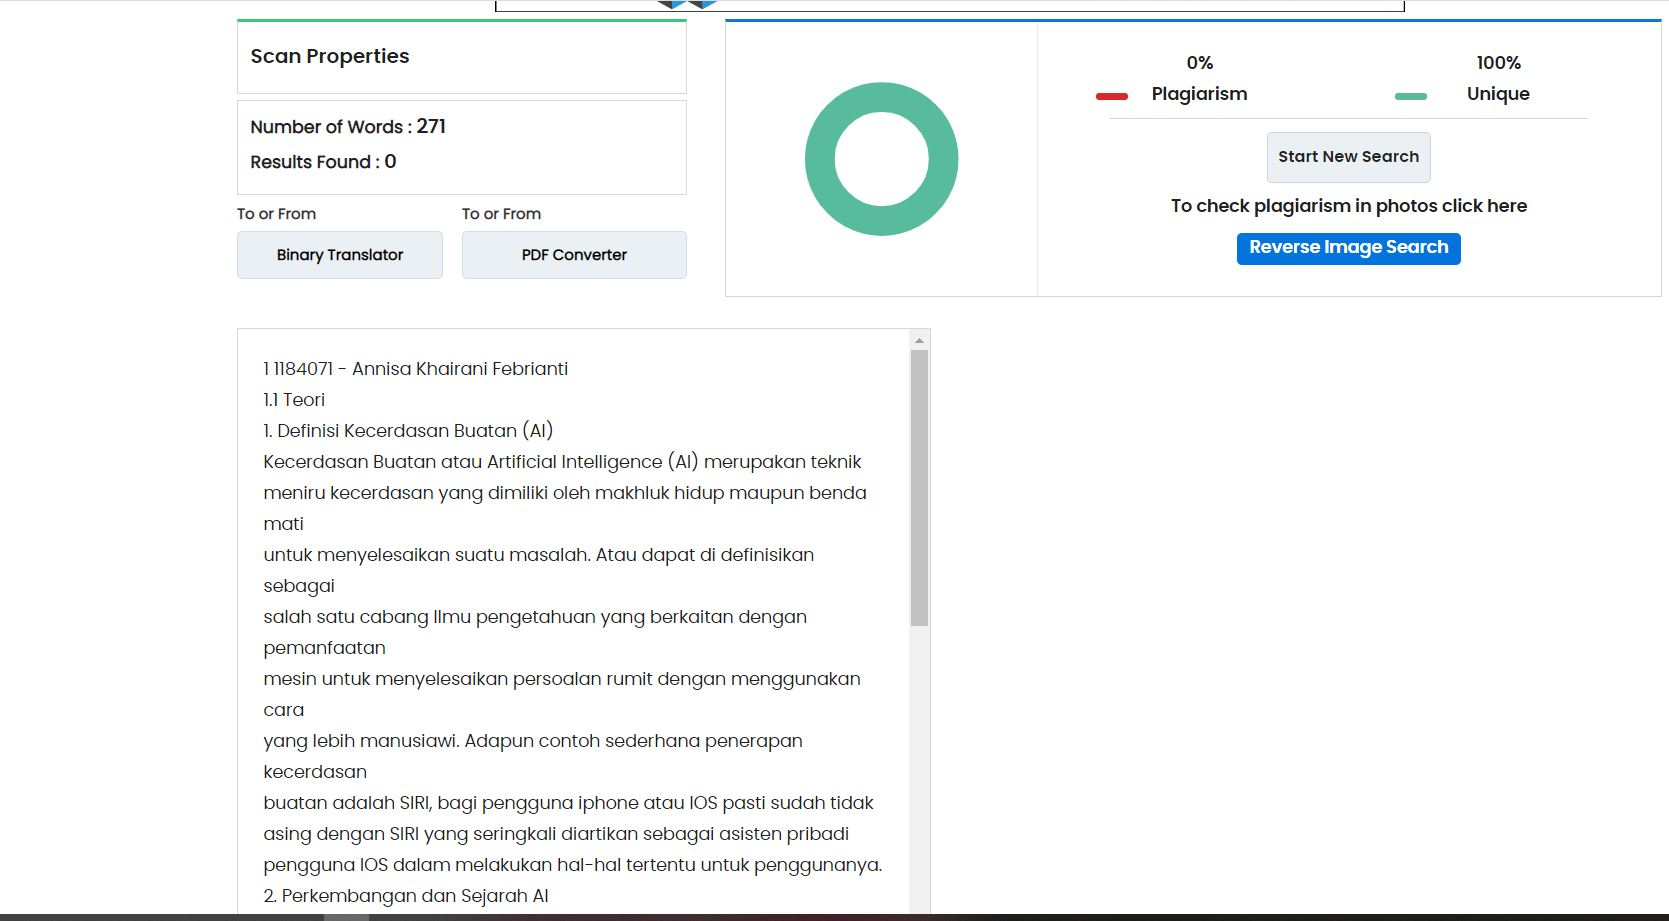
\includegraphics[width=15cm]{figures/1184071/chapter1/4.JPG}
	\centering
	\caption{Bukti Tidak Melakukan Plagiarisme Chapter 1}
\end{figure}